\documentclass[laboratorio]{guia}

\def \practnum {2} 
\def \practica {Conducci\'on el\'ectrica en l\'\i quidos}

\def \materia {Laboratorio de F\'\i sica II para Qu\'\i micos}
\def \periodo {2do. Cuatrimestre de 2015}
\def \catedra {Pablo Cobelli}
\def \website {http://materias.df.uba.ar/f2qa2015c2}
 
\usepackage{graphics}
\usepackage{amsmath}
\usepackage{amsfonts}
\usepackage{graphicx}
\usepackage{float}
\usepackage{wrapfig}
\usepackage{subfigure}
\usepackage{bm}
\usepackage{grffile}
\usepackage{color}
\usepackage{framed}
\usepackage[utf8]{inputenc}
\usepackage[T1]{fontenc}
\usepackage{lmodern}
\usepackage{circuitikz}
\usepackage[spanish]{babel}
\usepackage{babelbib}
\selectbiblanguage{spanish}

 

%----------------------------------------------------------
% Agrega al path de figuras el subdirectorio con el mismo
%     nombre que el archivo principal del proyecto
\graphicspath{{./\jobname/}}

%----------------------------------------------------------
% Definicion del entorno 'sabermas'
\makeatletter
\definecolor{shadecolor}{rgb}{0.89,0.91,0.94}
\newenvironment{sabermas}[1]{%
\vfill
\begin{shaded}
  \begin{center}
  {\textsection{Para saber m\'as}}
  \end{center}
  #1
\sf } 
{%
\end{shaded}%
}
\makeatother

%----------------------------------------------------------
% Definicion del entorno 'problema'
\newcounter{ContadorProblema}
\setcounter{ContadorProblema}{0}
\newcounter{TieneFiguraAsociada}
\setcounter{TieneFiguraAsociada}{0}
\newcounter{UbicacionFigura}
\setcounter{UbicacionFigura}{0}

\newenvironment{problema}[2][]
{%
    \ifx\relax#1\relax%
        \setcounter{TieneFiguraAsociada}{0}
        \else
        \setcounter{TieneFiguraAsociada}{1}
    \fi
    \def \archivofigura {#1}
    % 
    \refstepcounter{ContadorProblema}
    \noindent%
    \ifnum\value{TieneFiguraAsociada} < 1%
        {\sffamily \bfseries Problema \arabic{ContadorProblema}.}
        %{\sc {#1}}%
        \par\nobreak\par\nobreak%
        \medskip 
    \else
        % Va con figura; resta determinar de que lado.
        \ifnum\value{UbicacionFigura} < 1
            % Poner la figura del lado derecho
            \begin{minipage}{12.25cm}
            {\sffamily \bfseries Problema \arabic{ContadorProblema}.}
            %{\sc {#1}}%
            \par\nobreak\par\nobreak%
            \medskip 
        \else
            % Poner la figura del lado izquierdo
            \begin{minipage}{4.5cm}
                \centering
                \includegraphics[width=4.5cm]{\archivofigura}
                {\footnotesize {\sffamily Esquema asociado al 
                problema \arabic{ContadorProblema}}.}
            \end{minipage}\hfill%
            \begin{minipage}{12.25cm}
                {\sffamily \bfseries Problema \arabic{ContadorProblema}.}
                %{\sc {#1}}%
                \par\nobreak\par\nobreak%
                \medskip 
        \fi
    \fi
}
{%
    \ifnum\value{TieneFiguraAsociada} < 1%
        % \par \bigskip \vskip 0.3cm
    \else
        % Va con figura; resta determinar de que lado.
        \ifnum\value{UbicacionFigura} < 1
            % Poner la figura del lado derecho
            \end{minipage}\hfill%
            \begin{minipage}{4.5cm}
                \centering
                \includegraphics[width=4.5cm]{\archivofigura}
                {\footnotesize {\sffamily Esquema asociado al 
                problema \arabic{ContadorProblema}}.}
            \end{minipage}
        \else
            % Poner la figura del lado izquierdo
            \end{minipage}%
        \fi
    \fi
    \setcounter{TieneFiguraAsociada}{0}
    \par \bigskip \vskip 0.3cm
    % Permutamos el valor de la ubicacion
    \ifnum\value{UbicacionFigura} < 1
        \setcounter{UbicacionFigura}{1}
    \else
        \setcounter{UbicacionFigura}{0}
    \fi
}

%----------------------------------------------------------
% Definicion/Redefinicion de estilos
\renewcommand{\vec}[1]{\ensuremath{\mathbf{#1}}}



\hyphenation{ coe-fi-cien-tes coe-fi-cien-te au-to-va-lor
              au-to-va-lo-res co-rres-pon-der pro-ble-ma 
              cual-quie-ra po-la-ri-za-cio-nes }

\graphicspath{{./liquidos/}}

\begin{document} 
\objetivo{
  El objetivo de esta guía experimental es estudiar si los líquidos conducen o no la electricidad.
  Para aquellos que efectivamente conducen la electricidad, se propone estudiar la relación entre diferencia de potencial y corriente, a fin de establecer si satisfacen o no la Ley de Ohm. 
    \tematicas{Conducción, corriente, Ley de Ohm, materiales óhmicos y no-óhmicos.}
} 
\maketitle


\section{Introducción}
Para que un medio material pueda conducir la corriente eléctrica este debe contener cargas móviles capaces de conducir la electricidad.
En los metales, las cargas móviles son los mismos electrones de las capas más externas de los átomos que lo forman (electrones de conducción).
Al formarse el metal, el campo de cada átomo afecta a sus vecinos más próximos, lo que hace que los electrones más externos dejen de estar ligados a un solo átomo y tengan
libertad de moverse a través de todo el sólido.
En algunos líquidos, por ejemplo el agua, si se disuelven sales, ácidos o bases, estas se disocian en iones positivos y negativos que pueden moverse a través del líquido, por lo que la conducción eléctrica se hace apreciable.


\section{Conductividad de una solución salina}
El dispositivo experimental propuesto para el desarrollo de esta práctica se ilustra esquemáticamente en la figura \ref{fig:1}.
La tensión que suministra la fuente de tensión alterna (¿qué es una fuente de alterna?) es medida por un voltímetro conectado en paralelo.
Su valor puede variarse hasta \SI{20}{\volt}. 
\begin{figure}
    \centering
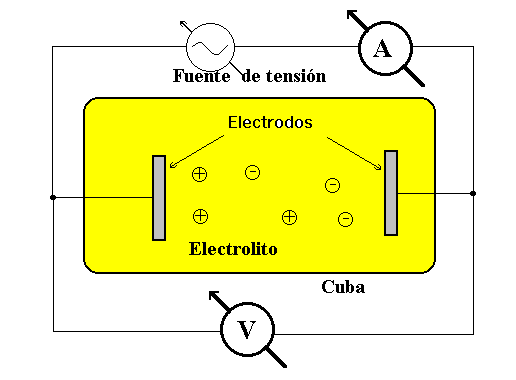
\includegraphics[width=8.5cm]{LG02b--001.png}
\caption{Esquema del dispositivo experimental propuesto (bandeja en vista superior).
La bandeja de material aislante contiene el electrolito bajo estudio.
La fuente suministra una diferencia de potencial alterna de amplitud controlable.
Con \(V\) se indica al voltímetro, y con \(A\) al amperímetro.}
\label{fig:1}
\end{figure}

Para verificar lo mencionado en la introducción, pruebe aplicando una diferencia de potencial alterna a una solución salina de agua en una cuba como la mostrada en la figura \ref{fig:1}.
Comience con sólo agua destilada en la cuba, aplique entonces una \(\Delta V\) alterna de unos \SI{10}{\volt} y mida la corriente \(I\) empleando un amperímetro.
Verifique que la conexión del amperímetro sea la adecuada para medir corriente alterna (modo AC). 

A continuación prepare una solución de \SI{1}{\gram} de sal común en \SI{0.5}{\litre} de agua.
Agregue a la cuba la solución de a una gota a la vez y vaya observando cómo varía la \(I\) que registra el amperímetro. 

Grafique los valores de corriente en función del número de gotas que introdujo en la cuba.
Grafique también \(I\) en función de la concentración en fracción molar (o en cualquier otra unidad de concentración que le parezca apropiada). 

Piense cómo afecta el número de portadores de carga (iones, en este caso) a la conductividad del medio electrolítico. 


\section{¿Responde el líquido a la Ley de Ohm?}
Usando una fuente de alterna, un voltímetro y un amperímetro estudie ahora cómo es la dependencia de la \(\Delta V\) con \(I\) en un líquido conductor.
Grafique sus resultados y, en función de la dependencia hallada, determine si el medio bajo estudio satisface o no la Ley de Ohm. 

En el caso de que el líquido conductor satisfaga efectivamente la Ley de Ohm, determine la resistencia \(R\) del sistema.




\nocite{Alonso1998,Purcell1988,Reitz1996}
\bibliographystyle{unsrt} 
\bibliography{Bibliografia}

\end{document}
